\documentclass[aspectratio=169]{beamer}
\usepackage[utf8]{inputenc}
\usepackage{hyperref}
\usepackage{amsmath,amsfonts,amsthm,bm}
\usepackage{color}
\usepackage{minted}
\usepackage{graphicx} % Allows including images
\usepackage{booktabs} % Allows the use of \toprule, \midrule and \bottomrule in tables
\usepackage{tikz}
\usepackage[version=3]{mhchem}
\usepackage{pgfplots}
\pgfplotsset{compat=1.16} 
\setminted{fontsize=\scriptsize}

\hypersetup{
    colorlinks=true,
    linkcolor=red,
    filecolor=magenta,      
    urlcolor=red,
}

\DeclareMathOperator*{\argmax}{argmax}
\DeclareMathOperator*{\argmin}{argmin}
\let \vec \mathbf

\newcommand{\classname}{NANOx81}
\newcommand{\classyear}{Fall 2023}
\mode<presentation> {
    \usetheme{CambridgeUS}
    \setbeamertemplate{footline}[text line]{%
      \parbox{\linewidth}{\vspace*{-8pt}\classname\hfill\classyear\hfill\insertpagenumber}}

    %\setbeamertemplate{footline}[page number]
    \setbeamertemplate{navigation symbols}{}
}


\title[Neural Networks]{Neural Networks}

\author{Shyue Ping Ong}
\institute[UCSD]{University of California, San Diego\\
\medskip
}
\date{\classyear} % Date, can be changed to a custom date

\begin{document}


\begin{frame}
    \titlepage % Print the title page as the first slide
\end{frame}


\begin{frame}{Overview}
    \tableofcontents
\end{frame}


\section{Preliminaries}

\begin{frame}{Preliminaries}
    \begin{itemize}
        \item Neural networks/deep learning has gotten a lot of hype in recent years.
        \item In many areas, they have outperformed many traditional ML methodologies.
    \begin{figure}
        \centering
        \includegraphics[width=0.45\textwidth]{figures/imagenet.pdf}
        \includegraphics[width=0.45\textwidth]{figures/alphago.jpg}
    \end{figure}
    \end{itemize}

\end{frame}

\section{Neural Networks}


\begin{frame}{Artificial Neural Network}
\begin{itemize}
        \item An artificial neural network (ANN) is a learning algorithm that is (very) loosely based on the structure of the brain.
        \item Somewhat vaguely, you will also hear the terms ``multi-layer perceptron'' (MLP) used in place of ANN.
        \begin{block}{Universal Approximation Theorem\cite{csajiApproximationArtificialNeural2001}}
        A feed-forward network with a single hidden layer containing a finite number of neurons can approximate continuous functions under mild assumptions on the activation function. 
        \end{block}
\end{itemize}
\begin{figure}
        \centering
        \includegraphics[width=0.4\textwidth]{figures/neuron.jpg}
    \end{figure}
\end{frame}


\begin{frame}{Neural Networks}
    \begin{figure}
    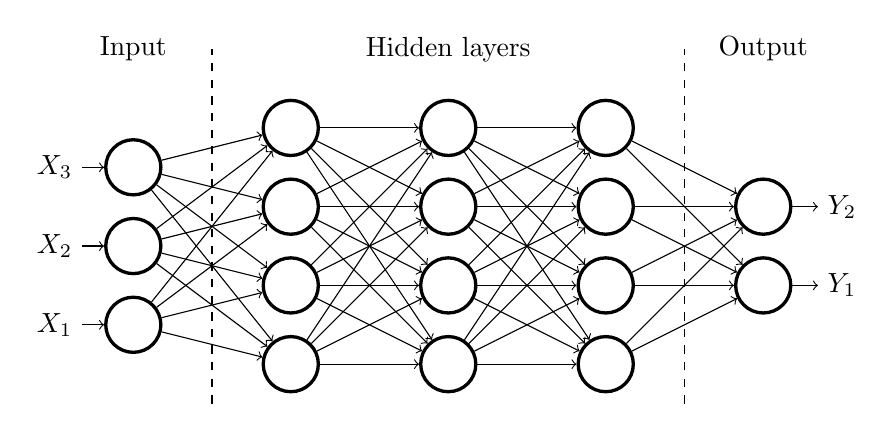
\begin{tikzpicture}[
        roundnode/.style={circle, draw=black, very thick, minimum size=7mm}
    ]
        \pgfmathsetmacro{\nin}{3}
        \pgfmathsetmacro{\nhl}{3}
        \pgfmathsetmacro{\nhn}{4}

        \foreach \i in {1,...,\nin}
        {
            \node at (-1, \i) (\i) {$X_\i$};
            \node[roundnode] at (0, \i) (i\i) {};
            \draw[->] (\i) -> (i\i);
        }

        \foreach \i in {1,...,\nhl}
        {
            \pgfmathsetmacro{\yshift}{(\nin - \nhl)/2}
            \foreach \j in {1,...,\nhn}
            {
                \node[roundnode] at (2*\i, -0.5+\j) (h\i\j) {};
            }
        }

        \foreach \i in {1,...,\nin}
        {
            \foreach \j in {1,...,\nhn}
            {
                \draw[->] (i\i) -- (h1\j);
            }
        }

        \foreach \i in {1,...,2}
        {
            \pgfmathtruncatemacro{\x}{\i +1};
            \foreach \j in {1,...,\nhn}
            {
                \foreach \k in {1,...,\nhn}
                {
                    \draw[->] (h\i\j) -- (h\x\k);
                }
            }
        }

        \foreach \i in {1,...,2}
        {
            \node[roundnode] at (8, 0.5+\i) (o\i) {};
            \foreach \j in {1,...,4}
            {
                \draw[->] (h3\j) -- (o\i);
            }
            \node at (9, 0.5+\i) (y\i) {$Y_\i$};
            \draw[->] (o\i) -- (y\i);
        }

        \draw [dashed] (1, 0) -- (1, 4.5);
        \draw [dashed] (7, 0) -- (7, 4.5);
        \node at (0, 4.5) {Input};
        \node at (4, 4.5) {Hidden layers};
        \node at (8, 4.5) {Output};
    \end{tikzpicture}
\end{figure}

\end{frame}


\begin{frame}{Neuron}
\begin{figure}
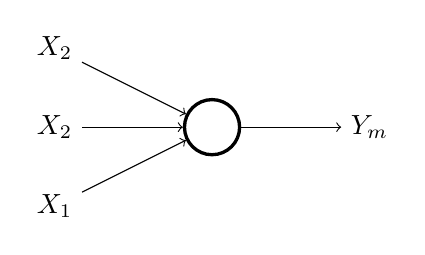
\begin{tikzpicture}
[roundnode/.style={circle, draw=black, very thick, minimum size=7mm}
]
\node at (0, 0) (X1) {$X_1$};
\node at (0, 1) (X2) {$X_2$};
\node at (0, 2) (X3) {$X_2$};
\node[roundnode] at (2, 1) (C) {};
\draw[->] (X1) -- (C);
\draw[->] (X2) -- (C);
\draw[->] (X3) -- (C);
\node at (4, 1) (Y) {$Y_m$};
\draw[->] (C) -- (Y);
\end{tikzpicture}
\end{figure}
\begin{equation*}
    Y_m = \sigma(\alpha_{0m} + \alpha_{m}^T \vec{X})
\end{equation*}
    \begin{itemize}
        \item Output of each neuron is a linear function of the inputs.
        \item In hidden layers, the output is passed through an \textit{activation function} $\sigma$.
        \item Common choices of $\sigma$ include the rectified linear unit (RELU), sigmoid function, softplus, etc.
    \end{itemize}
\end{frame}


\begin{frame}{Activation Functions}
\begin{figure}
    \centering
    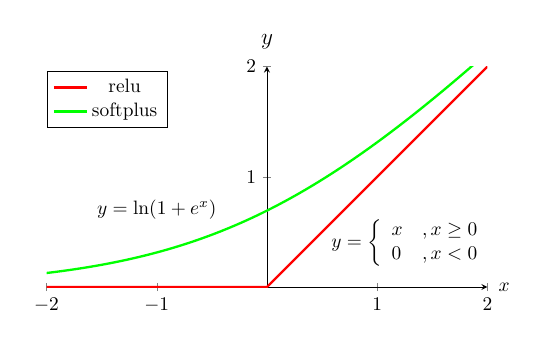
\begin{tikzpicture}[scale=0.7]
        \begin{axis}[
            axis lines=middle,
            inner axis line style={-stealth},
            xlabel={$x$},
            ylabel={\large $y$},
            ytick={0,1,...,2},
            xtick={-2,-1,...,2},
            y=2cm,
            x=2cm,
            x tick label style={below},
            y tick label style={left},
            x label style={at={(ticklabel* cs:1.01)},anchor=west},
            y label style={at={(ticklabel* cs:1.05)},anchor=south},
            ymin=0,
            ymax=2,
            xmin=-2,
            xmax=2,
            legend style={at={(0,0.85)},anchor=west}
        ]
        \addplot[color=red,very thick] coordinates {(-2, 0) (0, 0) (2, 2)};
        \addlegendentry{relu}
        \addplot[color=green,very thick,domain=-2:2,samples=100] {ln(1+exp(x))};
        \addlegendentry{softplus}
        \node at (axis cs:-1,0.7) {$y=\ln(1+e^x)$};
        \node at (axis cs:1.3,0.4) {$y=\left\{ \begin{array}{ll}
            x & , x \geq 0  \\
            0 & , x < 0
        \end{array} \right.$};
        \end{axis}
    \end{tikzpicture}
    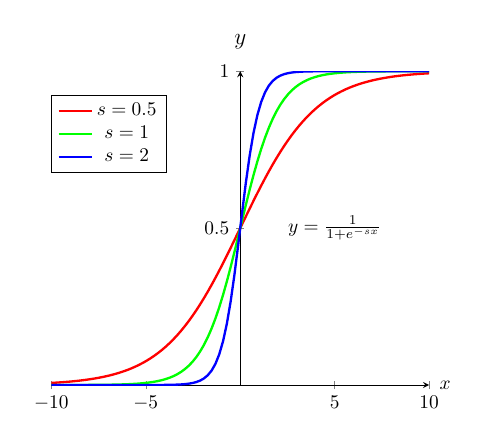
\begin{tikzpicture}[scale=0.7]
    \begin{axis}[
    axis lines=middle,
    inner axis line style={-stealth},
    xlabel={$x$},
    ylabel={\large $y$},
    ytick={0,0.5,1},
    xtick={-10,-5, 0,...,10},
    x label style={at={(ticklabel* cs:1.01)},anchor=west},
    y label style={at={(ticklabel* cs:1.05)},anchor=south},
    ymin=0,
    ymax=1,
    xmin=-10,
    xmax=10,
    legend style={at={(0,0.8)},anchor=west}
]
\addplot[color=red,very thick,domain=-10:10,samples=100] {1/(1+exp(-0.5*x))};
\addlegendentry{$s=0.5$}
\addplot[color=green,very thick,domain=-10:10,samples=100] {1/(1+exp(-x))};
\addlegendentry{$s=1$}
\addplot[color=blue,very thick,domain=-10:10,samples=100] {1/(1+exp(-2*x))};
\addlegendentry{$s=2$}
\node at (axis cs:5,0.5) {$y=\frac{1}{1+e^{-sx}}$};
\end{axis}
    \end{tikzpicture}
\end{figure}
\end{frame}


\begin{frame}{Fitting a Neural Network}
    \begin{itemize}
        \item Model \textit{weights} ($\alpha$ in the linear functions) are fitted by \textit{back-propogation}, basically a form of gradient descent.
        \item Loss functions: squared error for regression, squared error or cross entropy for classification.
        \item To avoid overfitting, regularization (similar to ridge regression) is typically applied. E.g., \textit{weight decay}:
        \begin{equation*}
            J = \sum \alpha^2
        \end{equation*}
    \end{itemize}
\end{frame}


\begin{frame}{Parameter Decisions for Neural Networks}
    \begin{itemize}
        \item Number of hidden units and layers: generally error on the side of having too many hidden units than too few - flexibility is needed to capture non-linearities in the data.
        \item Extra weights can be shrunk to zero with appropriate regularization.
        \item Learning rate is a key parameter in fitting ANNs as well as other models. The learning rate controls the rate of gradient descent. A high learning rate reduces training time, but also decreases accuracy. State-of-the-art is to use an adaptive learning rate. 
        \item The error function is non-convex and contains multiple minima, i.e., final solution obtained depends on initial weights. Typical approach is to start with a number of random starting configurations and choose solution with lowest penalized error.
        \item Alternative is to average predictions over a number of ANN, i.e., ensemble models.
    \end{itemize}
\end{frame}


\begin{frame}{Software packages for Neural Networks}
    \begin{itemize}
        \item Scikit-learn has a basic implementation of a multi-layer perceptron. For this course, we will use this to avoid overloading students with different software packages.
        \item However, you should be aware that if you are into serious work with ANNs, alternative software are available that offer more features and efficiency. Note that these packages are not limited to ANNs, but ANNs are the most common use case.
        \begin{itemize}
            \item \href{https://www.tensorflow.org/}{Tensorflow}. Open-source package by Google. Very powerful and efficient, but a very steep learning curve. Highly recommend that you use the Keras package (already integrated into TF2) which provides a high level API to it similar to scikit-learn in some ways.
            \item \href{https://pytorch.org/}{Pytorch}. Open-source package by Facebook. Equally powerful as TF but also steep learning curve.
        \end{itemize}
    \end{itemize}
\end{frame}


\begin{frame}[fragile]{ANNs in Scikit-learn and TF2.0}
\inputminted{python}{example_sklearn_tf_neural_network.py}
\end{frame}


\begin{frame}{Beyond the Feedforward Neural Network}
    \begin{itemize}
        \item ANNs can be an entire course in itself. Here, we cover some basic variations.
        \begin{description}
        \item[Convolutional NNs] Uses covolutional operations to achieve translational invariance. Especially important in image processing applications. In modeling crystals with periodic boundary conditions, this can also be a useful feature.
        \item[Recurrent NNs] Connections between nodes form a directed graph along a temporal sequence. Exhibits temporal dynamic behavior and can handle variable length sequences of inputs. Applications: handwriting recognition or speech recognition.
        \end{description}
        
    \end{itemize}
\end{frame}


\section{Applications}


\begin{frame}{Example Application: NN for interatomic potentials}
    \begin{itemize}
        \item Atom-centered symmetry functions (ACSF)\cite{behlerAtomcenteredSymmetryFunctions2011} to represent the atomic local environments.
        \begin{eqnarray*}
            G_{i}^{\rm atom, \rm rad} & = & \sum_{j\neq i}^{N_{\rm atom}} e^{-\eta(R_{ij}-R_{s})^{2}} \cdot f_{c}(R_{ij}), \\
            G_{i}^{\rm atom, \rm ang} & = & 2^{1-\zeta}\sum_{j,k \neq i}^{N_{\rm atom}} (1 + \lambda \cos \theta_{ijk})^{\zeta} \cdot e^{-\eta^{\prime}(R_{ij}^{2}+R_{ik}^{2}+R_{jk}^{2})}\cdot\\
            & & f_{c}(R_{ij}) \cdot f_{c}(R_{ik}) \cdot f_{c}(R_{jk}),
        \end{eqnarray*}
        where $R_{ij}$ is the distance between atom $i$ and neighbor $j$; $\eta$ is the width of the Gaussian; $R_{s}$ is the position shift over all neighboring atoms; $\zeta$ controls the angular resolution. $f_{c}(R_{ij})$ is a cutoff function.    
        \item Fully connected ANNs describe the PES with respect to ACSFs.\cite{behlerHighDimensionalNeuralNetwork}
        \item Has been developed for Si, \ce{TiO2}, water, metal-organic frameworks, ZnO, \ce{Li3PO4}, etc.
    \end{itemize}
\end{frame}


\begin{frame}{Example Application: NNP for Si}
    \begin{figure}
        \centering
        \includegraphics[width=0.45\textwidth]{figures/nnp.pdf}
        \includegraphics[width=0.45\textwidth]{figures/nnp-si.pdf}
        \caption{Left: Schematic of NNP architecture. Right: Comparison of radial distribution functions from MD simulations using various interatomic potentials for Si.\cite{behlerGeneralizedNeuralNetworkRepresentation2007}}
        \label{fig:my_label}
    \end{figure}
\end{frame}




\begin{frame}{Example Application: NNP-computed phase diagram for amorphous Li-Si}
\begin{figure}
    \centering
    \includegraphics[width=0.45\textwidth]{figures/li-si-nnp.pdf}
    \includegraphics[width=0.5\textwidth]{figures/li-si-nnp2.pdf}
    \caption{From ref \cite{artrithConstructingFirstprinciplesPhase2018}}
\end{figure}
\end{frame}


\begin{frame}{Example application: ANNs to predict crystal stability}
\begin{figure}
    \centering
    \includegraphics[width=0.35\textwidth]{figures/dnn-crystal-stability.png}
    \includegraphics[width=0.35\textwidth]{figures/dnn-crystal-stability2.png}
    \caption{ANNs predict formation energies of garnets and perovskite crystals from Pauling electronegativity and ionic radii.\cite{yeDeepNeuralNetworks2018}}
\end{figure}
\end{frame}


\begin{frame}{Example application: CNNs for determination of crystal symmetry from electron diffraction}
\begin{figure}
    \centering
    \includegraphics[width=0.4\textwidth]{figures/science-cnn-electron-diffraction.jpg}
    \includegraphics[width=0.25\textwidth]{figures/science-cnn-electron-diffraction2.jpg}
    \caption{CNNs to determine crystal symmetry from electron diffraction patterns with $>$ 90\% accuracy.\cite{kaufmannCrystalSymmetryDetermination2020}}
\end{figure}
\end{frame}


\begin{frame}[allowframebreaks]{Bibliography}
    \bibliographystyle{unsrt}
    \bibliography{refs}
\end{frame}


\begin{frame}
    \Huge{\centerline{The End}}
\end{frame}

\end{document}

